% !TeX root = ../main.tex
% Add the above to each chapter to make compiling the PDF easier in some editors.

\chapter{Simulator Choice}


Simulator choice was the first important architecture decision we made, because it influences the whole software architecture. Simulator lays the groundwork of the robotics environment implementation. 
Especially for continuous control optimization tasks, accurate simulation plays a significant role in the performance of the controller. As Todorov et al. indicated, if the simulation is not accurate enough, an optimization algorithm will find a way to exploit it \cite{Todorov2012}.
We compared three states of art simulators: Mujoco\footnote{\url{http://www.mujoco.org/}}, Gazebo\footnote{\url{http://gazebosim.org/}}, and Pybullet\footnote{\url{https://pybullet.org/}}. Each simulator comes with advantages and drawbacks. Our decision is based on the factors: active support, community, stability, scalability, and ease of use. It is important to note that our analysis includes subjective factors such as ease of use, documentation coverage, and tutorials quality. Although we tried our best to ground our points on facts, subjective criteria include a certain amount of personal preferences. 

\subsection{Mujoco}

Mujoco is released in 2015, making it the newest physics engine in our comparison. It stands for Multi-Joint Control. Hence the name, its primary purpose is Robot simulation.
 
We first considered Mujoco as our main simulator. Our consideration was based on; Roboticist mainly using Mujoco at OpenAI and DeepMind \cite{OpenAIgym}. In addition, simulation engine reviews featured Mujoco as the best performing and stable engine \cite{Erez2015}. Erez et al. conducted tests that compared the performance of physics engines on grasping tasks, where Mujoco by far performed better than the other engines \ref{fig:handmujoco}. Additionally, Mujoco provides an API that lets users develop in C language. C language API is a significant advantage for researchers aim to get as close to the hardware as possible to save time. Another plus is mujoco-py offers a Python API to control Mujoco simulation easily. OpenAI product Mujoco-py\footnote{\url{https://github.com/openai/mujoco-py}} is entirely open-source with MIT license. 

\begin{figure}[htbp]
    \centering
      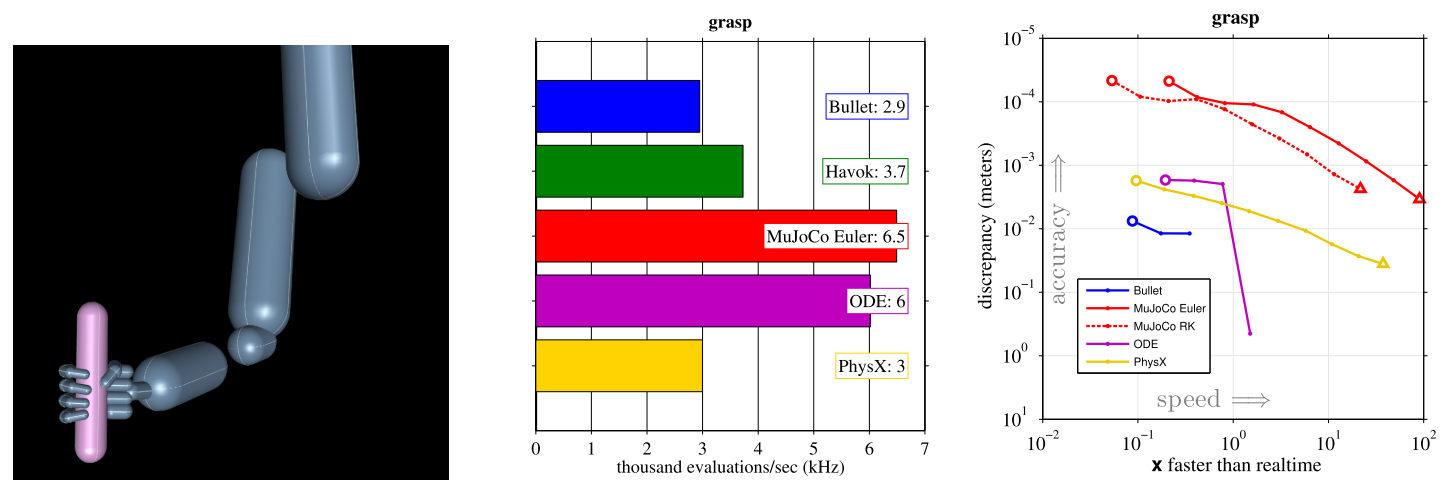
\includegraphics[width=1.0\textwidth]{figures/MujocoHand}
    \caption{physics engine performance on grasping task. Mujoco performs the best \cite{Erez2015}}
    \label{fig:handmujoco}
\end{figure}


On the other hand, MuJoCo requires a license to use for research purposes. Personal non-commercial license costs \(500\$\) as of 2020 July. License cost is the main drawback because we prefer complete open-source software. Another factor is the training time since our models require over 10M time-steps to train, we need to make use of every millisecond time gain in every step. So, GPU support is highly crucial. Mujoco only supports CPU simulation, which has the potential to be slower than GPU. As a side-note, we have not compared the MuJoCo CPU version speed with Bullet GPU version speed. MuJoCo developers prepared a performance page where they explain the GPU vs. CPU comparison. They pointed out that if decoupled systems are to be simulated like particle simulation, GPU has an advantage. Whereas, one simulates coupled system such as a humanoid robot CPU gain a slight edge \ref{fig:mujococpu}. They also noted that there is room for research in the areas besides coupled or decoupled systems\footnote{\url{http://mujoco.org/performance.html}}.

\begin{figure}[htbp]
    \centering
      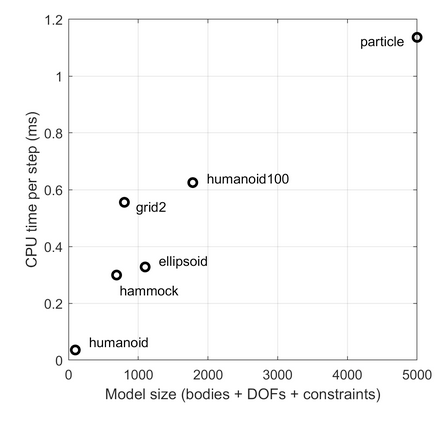
\includegraphics[width=0.7\textwidth]{figures/MujocoCPU1}
    \caption{CPU time per step comparison of different tasks \cite{Erez2015}}
    \label{fig:mujococpu}
\end{figure}

Finally, observing large open-source projects like OpenAI-Roboschool, which initially used MuJoCo, deprecating, and suggesting PyBullet, made us reconsider. We believe that the reason community migrating towards PyBullet is completely open-source codebase. 

\begin{figure}[htbp]
    \centering
      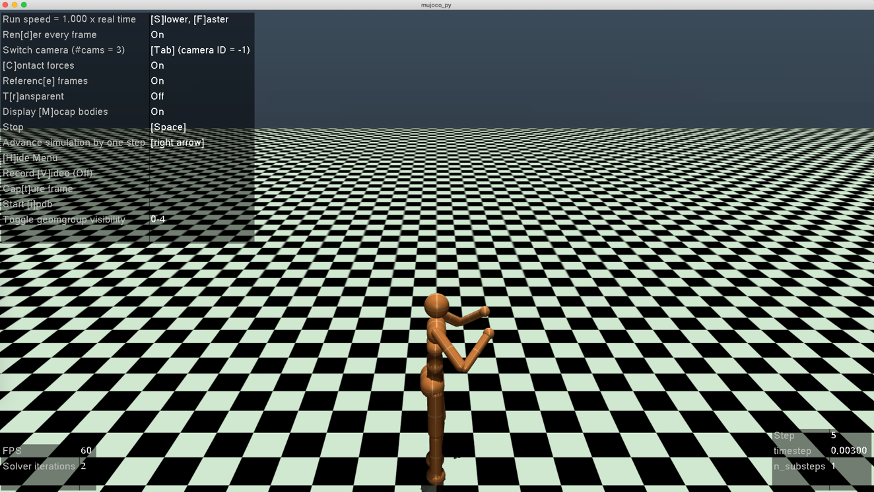
\includegraphics[width=1.\textwidth]{figures/MujocoHuman1}
    \caption{Mujoco simulation of a humanoid model. Rendered with MJViewer}
    \label{fig:mujocohuman}
\end{figure}

\subsection{Gazebo}

The Gazebo is the oldest simulator among Bullet and Mujoco. The development of Gazebo dates back to the 2002 University of Southern California. Later, Willow Garage took over and extended Gazebo to ROS and PR2. Gazebo became the primary simulation engine of the ROS community. Eventually, in 2012 Gazebo became part of OSRF (Open Source Robotics Foundation)\footnote{\url{https://www.openrobotics.org/}}, a spin-off from Willow Garage.

Technically, Gazebo is a simulation platform, which inherits different physics engines, such as Bullet, ODE\footnote{\url{https://www.ode.org/}}, Simbody\footnote{\url{https://simtk.org/}}, and DART\footnote{\url{https://dartsim.github.io/}}. According to the documentation of Gazebo 11.0, it supports ODE engine default, and other engines can be used if developers compile Gazebo from the source. That means the performance of the overall Gazebo simulation highly depends on those individual physics engine’s performances.  Another dependency of Gazebo is ROS (Robotics Operating System)\footnote{\url{https://www.ros.org/}}. ROS infrastructure handles all communication. Thus, users need to rely on ROS to interact with Gazebo. We believe this assumption is too large. Even if relying on ROS can bring many well-structured tools, learning ROS has a steep curve and can cause a large overhead for simple projects.
Nonetheless, developers invested highly on neat and clean documentation to reduce the overhead for new users. We consider the documentation and tutorials as a merit of the open-source project. Correspondingly, being open source contributes hugely to a large community willing to support, answering questions on forums, and submitting pull requests for possible bug fixes. 

According to Pitonakova et al., Gazebo has usability issues due to not having a 3D mesh editing option and difficulties of installing dependencies for third party models. They also noted that Gazebo performs reasonably well in large simulation environments, so it could be more convenient to conduct extensive swarm robotics experiments on Gazebo \cite{Pitonakova2018}.  

Based on our experiments in \ref{fig:GazeboPR2}, we found that Gazebo provides useful models to set up a table-top environment for robotics picking applications quickly. Although we have not performed any grasping experiments on Gazebo, editing the size, position, and orientation of models directly on simulation GUI is a useful feature, lacking both on Pybullet and Mujoco.


\begin{figure}

    \begin{subfigure}{0.49\textwidth}
      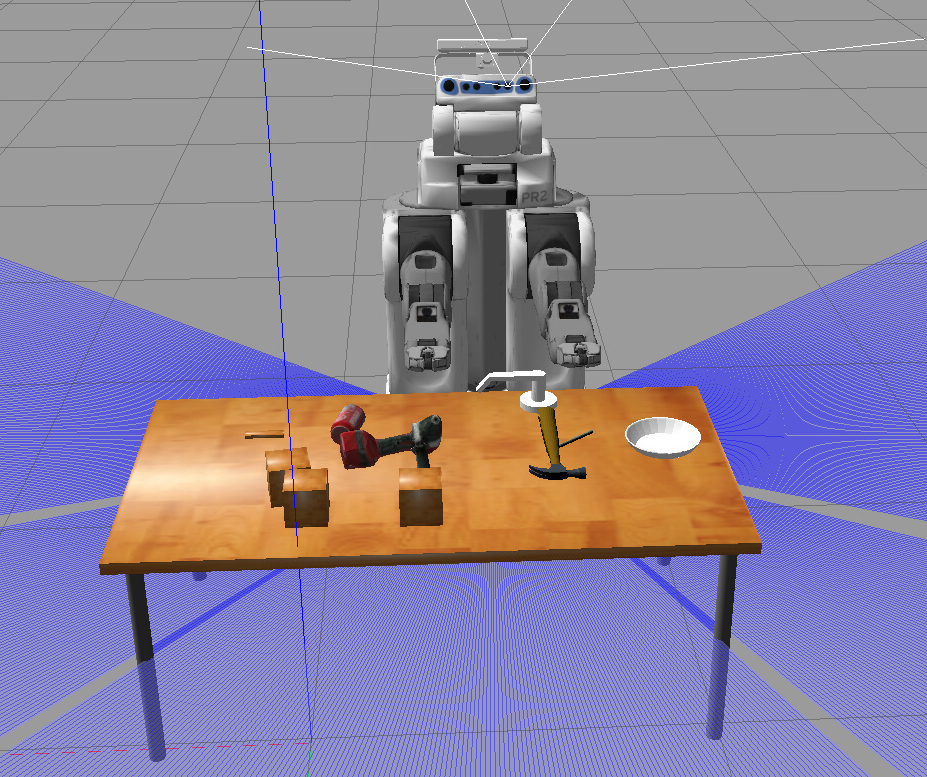
\includegraphics[width=\linewidth]{figures/GazeboEnv1.png}
      \caption{} \label{fig:1a}
    \end{subfigure}%
    \hspace*{\fill}   % maximize separation between the subfigures
    \begin{subfigure}{0.49\textwidth}
      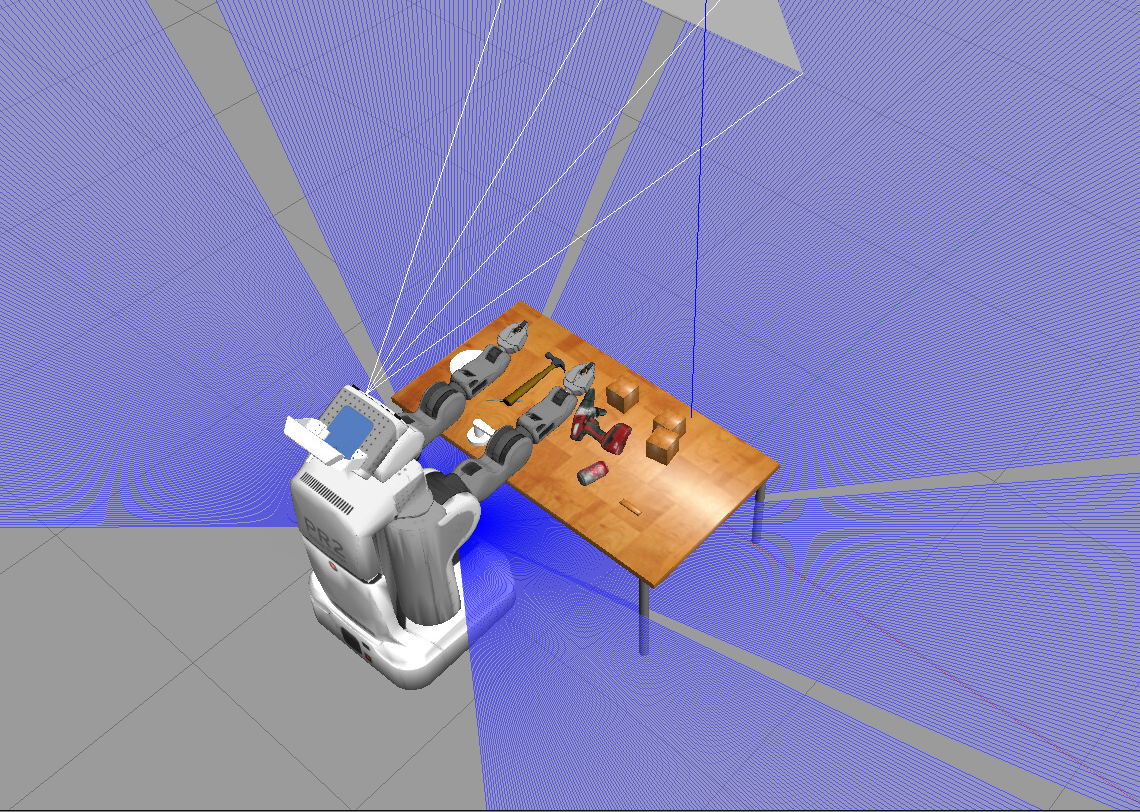
\includegraphics[width=\linewidth]{figures/GazeboEnv2.png}
      \caption{} \label{fig:1b}
    \end{subfigure}%

\caption{Table-top environment in Gazebo simulation with variety of objects and PR2 robot \label{fig:GazeboPR2}}
\end{figure}

\subsection{PyBullet}

PyBullet is a simulator built on the Bullet physics engine. Bullet’s initial release dates back to 2006. Bullet engine was initially game, and graphics focused, but lately, with PyBullet, it has been increasingly popular among roboticists. We decided on using PyBullet for several strong reasons and overall satisfied by the performance and the features it offers. Firstly, PyBullet recently published their RL resources on Github \footnote{\url{https://bit.ly/3h1X7uU}}. These resources provide everything necessary to quickly start experimenting with any choice of robot, environment, and algorithm. Secondly, in the area of RL robotics research, our reference papers are using PyBullet for their experiments \cite{Quillen2018} \cite{Breyer2018}. Therefore, it is more convenient to compare results using the same physical engine to avoid simulation differences. Thirdly, it has sizeable open-source support and free to use. 

On the other hand, based on Erez et al. performance tasks, which compares Bullet, Mujoco, ODE, and PhysX engines, Bullet is either at the last place or the one above the last position \ref{fig:BulletComp} figure. Similarly, they mention the incompatibility of Bullet Engine’s spring-damper system with the standard PD controller design \cite{Erez2015}.

Many open-source robotics learning resources migrating to PyBullet. This migration brings more open-source contributors who are more focused on Reinforcement Learning. For example, open-source contributors recently developed multi-threading GPU support to PyBullet. Also, stable-baselines\footnote{\url{https://github.com/hill-a/stable-baselines}} creators implemented a RL training package under Bullet’s Github repository\footnote{\url{https://bit.ly/3jqU7Kd}} \cite{stable-baselines}. 

In conclusion, PyBullet is the most actively developed physics engine among three contenders. Thanks to the open-source community, any small bug is reported and solved quickly, which is missing in Gazebo and Mujoco. We assume more roboticists will migrate to PyBullet in the future. As a result of this, it will become a primary physics engine for robotics research. Despite research papers representing Pybullet engine performance as the worst among three, we have not noticed any significant failure related to engine performance in practice.

\begin{figure}

    \begin{subfigure}{0.31\textwidth}
      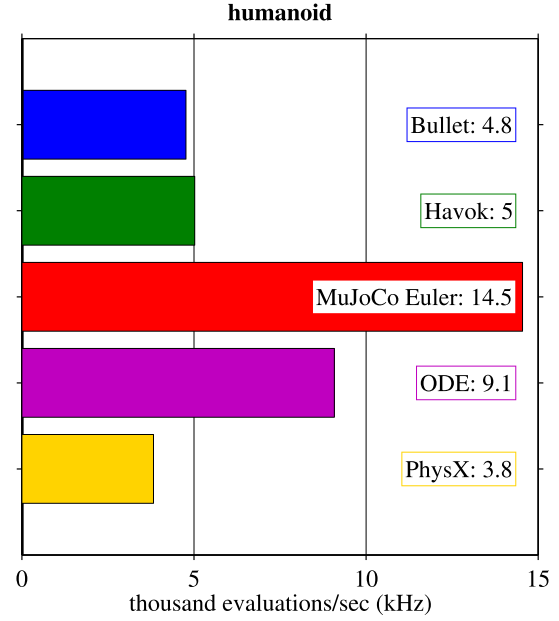
\includegraphics[width=\linewidth]{figures/BulletCom1.png}
      \caption{} \label{fig:1a}
    \end{subfigure}%
    \hspace*{\fill}   % maximize separation between the subfigures
    \begin{subfigure}{0.31\textwidth}
      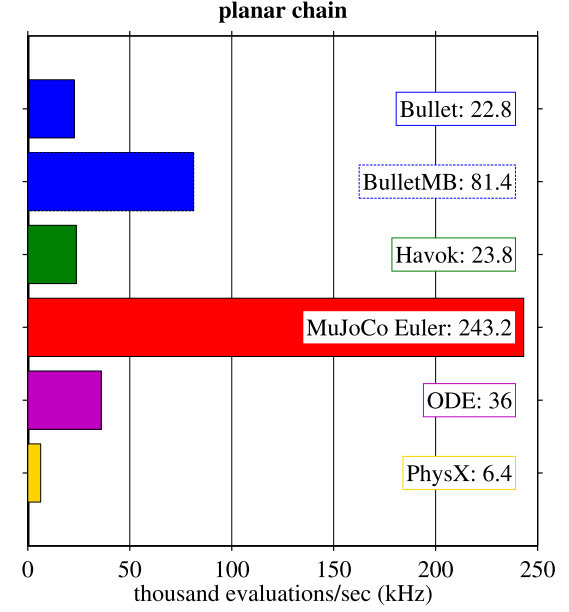
\includegraphics[width=\linewidth]{figures/BulletCom2.png}
      \caption{} \label{fig:1b}
    \end{subfigure}%
    \hspace*{\fill}   % maximize separation between the subfigures
    \begin{subfigure}{0.31\textwidth}
      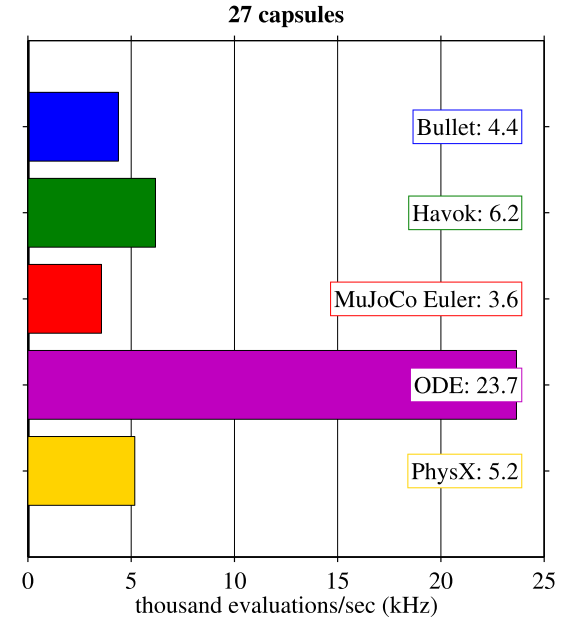
\includegraphics[width=\linewidth]{figures/BulletCom3.png}
      \caption{} \label{fig:1b}
    \end{subfigure}%

\caption{Comparing physics engine performances. Bullet is either at the last place or the one above the last position \cite{Erez2015} \label{fig:BulletComp}}
\end{figure}


\begin{figure}

    \begin{subfigure}{0.49\textwidth}
      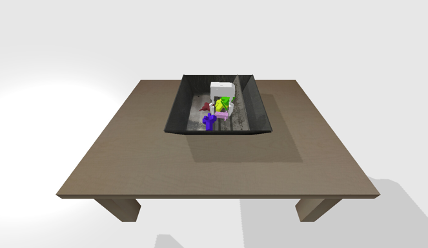
\includegraphics[width=\linewidth]{figures/PybulletEnv1.png}
      \caption{} \label{fig:1a}
    \end{subfigure}%
    \hspace*{\fill}   % maximize separation between the subfigures
    \begin{subfigure}{0.49\textwidth}
      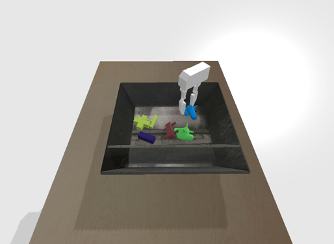
\includegraphics[width=\linewidth]{figures/PybulletEnv2.png}
      \caption{} \label{fig:1b}
    \end{subfigure}%

\caption{Screenshot from our trained hand model in Pybullet \label{fig:gripperbullet}}
\end{figure}



\begin{table}[h]
    \centering
    \begin{tabular}{|l|l|l|l|}
    \hline
    \textbf{Simulator}     & \textbf{Gazebo} & \textbf{MuJoCo} & \textbf{Pybullet}       \\ \hline
    \textbf{Designed For}  & Robotics        & Robotics        & Graphics/Games/Robotics \\ \hline
    \textbf{License}       & Open-Source     & Closed-Source   & Open-Source             \\ \hline
    \textbf{API}           & C++/Python      & C               & Python                  \\ \hline
    \textbf{Documentation} & 4/5             & 3/5             & 5/5                     \\ \hline
    \textbf{Ease of Use}   & 2/5             & 3/5             & 5/5                     \\ \hline
    \end{tabular}
    \caption{Comparison of simulators. Finally, we decided on PyBullet}
    \label{tab:simulation}
\end{table}